\chapter{Theory}
  \section{Introduction}
    Microseconds after the big bang, the universe existed in a state known as
      the Quark Gluon Plasma (QGP).
    In the QGP, quarks and gluons are not in hadronic bondage, forced to 
      the confines of bound states such as protons and neutrons.
    The Large Hadron Collider (LHC) produces QGP in the lab in PbPb (lead-lead)
      collisions.
    The high energies and rates of the collisions at the LHC make it possible 
      to do detailed studies of the QGP. 
    The LHC is producing rare experimental probes such as suppressed jets and 
      heavy quarkonia at an unprecedented rate in heavy-ion collisions. 
    Physicists now have better constraints on the properties like temperature,
      viscosity, and energy density of the QGP. 
    
    The detailed studies of PbPb collisions coming out of the LHC 
      experiments require an understanding of the initial state of the ions 
      before they collide.
    Without knowledge of the initial state, physicists cannot determine which
      experimental effects are due to the QGP and which effects are inherent to
      the nuclei themselves. 
    For example, suppression of heavy quarkonia is a signature of the QGP 
      but also appears to occur in deuterium-gold collisions where the QGP is not
      expected to arise \cite{dAuOniaPHENIX}. 
    Because it is not certain how much of the reduction of quarkonia production
      is due to the initial state of the nuclei, the reduction due to the QGP
      is unclear. 
    Without a clean probe of the initial state, physicists' knowledge of the 
      QGP is limited.
    Ultra-Peripheral Collisions (UPC) at the LHC fill this need for a clean 
      probe. 

    The colliding nuclei interact electromagnetically in an UPC event, avoiding
      the complicated mixing of final state and initial state effects found 
      in nuclear collisions.
    In UPC events, no QGP state emerges, and the effects arising from the QGP 
      no longer obscure the initial state effects.
    Other initial state probes such as peripheral nuclear collisions and 
      proton-nucleus collisions have the potential to create the QGP obscuring 
      which effects come from the initial state.
    It is impossible to create the QGP in UPC events because the nucleons 
      within the nucleus do not collide. 
    UPC events provide clarity by enhancing physicists' 
      understanding of the initial state. 
    
    The interactions between the field of photons surrounding the colliding 
      nuclei and the gluons of nuclei can produce a $J/\psi$ probing the 
      gluon density.
    The UPC $J/\psi$ photoproduction cross section is therefore a probe of 
      the initial state of the nucleus. 
    The Weizsi\"{a}cker-Williams approximation provides a way to calculate the 
      density of probing photons that surrounds the nucleus. 
    The electron-proton scattering data gives a value for the proton 
      photoproduction cross section at lower energies.
    The perterbutive Quantum Chromo-dynamics (pQCD), Vector Messon Dominance 
      (VMD), and Leading Twist (LTA) methods all combined the nuclear photon 
      flux with the proton scattering data to calculate the nuclear 
      photoproduction cross section.
    Each of these methods handle the gluon density of the nucleus differently 
      producing a measurable difference in the value of the $J/\psi$ 
      photoproduction cross section. 


  \section{QCD/QGP}


  \section{CGC/intial state}


  \section{Weizs\"{a}cker-Williams Approximation}
    The Weizsi\"{a}cker-Williams approximation relates the electric field of a 
      stationary point charge to the photon field that arises at ultra 
      relativistic velocities. 
    The approximation is semi-classical and combines both classical and quantum 
      elements.
    A Fourier transform of Maxwell's equations combine with Einstein's equation 
      for the energy of a photon in the Weizsi\"{a}cker-Williams approximation.
    \begin{wrapfigure}{r}{0.75\textwidth}
      \begin{center}
        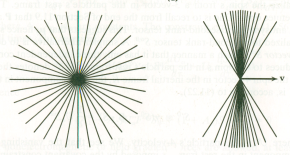
\includegraphics{boost.png}
      \end{center}
      \caption{ \label{fig:boost} The electromagnetic field boosted and at rest. }
    \end{wrapfigure}
    The frequency modes of the electrostatic field are treated as photons. 
    The conversion of the electric field to a flux of photons simplifies the
      calculation of interaction cross sections. 
    The Weizsi\"{a}cker-Williams approximation makes the calculation of 
      electromagnetic interactions with the nucleus tractable. 

    The Wiezacker-Williams approximation begins with the equation for the 
      electric field of the projectile nucleus at rest. 
    The electromagnetic field only needs to be considered at the position of 
      the target nucleus. 
    From the projectile's point of view, the target is moving and contributes
     $-vt$ to Eq.~\ref{eq:staticEFromTargtmp}, the equation for the electric 
     field of the projectile nucleus at rest.
    \begin{equation} \label{eq:staticEFromTargtmp}
        x'=-vt'\qquad
        y'=b\qquad
        z'=0\qquad
	\vec{\mathbf{E'}}=\left(\frac{eZ}
         {4 \pi \epsilon_{0}\left(\left(-vt'\right)^{2}+b^{2}\right)^{3/2}}\right)
	 \left(-vt'{\mathbf{\hat{x'}}+b\mathbf{\hat{y'}}}\right)
    \end{equation}        
    In Eq.~\ref{eq:staticEFromTargtmp}, $b$ is the impact parameter, 
      the distance of separation at closest approach, $v$ is the velocity of the 
      projectile nucleus, $Z$ is the number of protons in the nucleus, and $e$ 
      is the charge of the electron.
    Two simplifications occur due to the coordinates of 
      Eq.~\ref{eq:staticEFromTargtmp}.
    The magnetic field is equal to zero, because the projectile is at rest, and
      the $z$ coordinate can be ignored, reducing the equation to two dimensions. 

    The Lorentz transformation converts the field equations in the 
      projectile's frame to equations in the target's frame.
    The result is a set of equations that relate the electric and magnetic field
      components in one frame to the components of the electric and magnetic 
      field in another frame moving at a different constant velocity.
    Eq.~\ref{eq:staticEFromTarg2tmp} gives the result of the transformation 
      from the projectile's primed frame to the target's rest frame for 
      the field components \cite{WWJackson}:
    \begin{eqnarray} \label{eq:staticEFromTarg2tmp}
        E_{x}'=E_{x}\qquad
        \gamma\left(E_{y}'/c+\beta B_{z}'\right)=E_{y}/c\qquad
        \gamma\left(E_{z}'/c=\beta B_{y}'\right)=E_{z}/c \nonumber \\
        B_{x}'=B_{x}\qquad
        \gamma\left(B_{y}'-\beta E_{z}'/c\right)=B_{y}\qquad
        \gamma\left(B_{z}'+\beta E_{y}'/c\right)=B_{z}
    \end{eqnarray}
    The transformation equations for the fields, 
      Eq.~\ref{eq:staticEFromTarg2tmp}, and the transformation of the 
      coordinates reduce to Eq.~\ref{eq:staticEFromTarg3tmp} \cite{WWJackson}:
    \begin{eqnarray} \label{eq:staticEFromTarg3tmp}
        E_{x}'=E_{x}\qquad
        \gamma E_{y}'=E_{y}\qquad
        \gamma \beta E_{y}'/c=B_{z}\nonumber \\
        ct'=\gamma ct \qquad
        x'=-\gamma \beta c t
    \end{eqnarray}
    The simplicity of Eq.~\ref{eq:staticEFromTargtmp} creates the simplicity of
      Eq.~\ref{eq:staticEFromTarg2tmp}.
    The Lorentz transformation reduces the six components of the 
      electromagnetic field in the target's frame to the three equations in 
      Eq.~\ref{eq:staticEFromTarg2tmp} by relating them to the fields of the 
      projectile's frame. 
    
    The combination of Eq.~\ref{eq:staticEFromTargtmp} and 
      Eq.~\ref{eq:staticEFromTarg2tmp} produce equations for the electric and 
      magnetic fields in the target's rest frame. 
    Eq.~\ref{eq:staticEFromTargtmp} gives the expression for the field 
      components as seen in the projectile frame. 
    \begin{eqnarray} 
	\vec{\mathbf{E}}=\left( \frac{\gamma e Z}
         { 4 \pi \epsilon_{0} \left( \left( \gamma v t \right)^{2} 
	 + b^{2}\right)^{3/2} }\right)
         \left(vt\mathbf{\hat{x}}+b\mathbf{\hat{y}}\right)\qquad\nonumber \\
	 \vec{\mathbf{B}}=\frac{\gamma\beta e Z b}
	 { 4 \pi c \epsilon_{0} \left( \left( \gamma v t \right)^{2} 
	 + b^{2}\right)^{3/2} }
         \mathbf{\hat{z}}=
	 \frac{\gamma\mu_{0}veZb}{4\pi\left(\left(\gamma v t \right)^{2}
	 +b^{2}\right)^{3/2}}\mathbf{\hat{z}}
    \end{eqnarray}
    If the impact parameter $b$ goes to zero, the target sits in the line of 
      the projectile particle's motion, and the denominator carries a factor of
      $\gamma$ squared. 
    If $vt$ goes to zero, the projectile particle is directly above or below in
      the $y$ direction, and the numerator carries a factor of $\gamma$. 
    This results in fields that are a factor of $\gamma^3$ higher in the 
      $y$ direction than in the $x$ direction (see Fig.~\ref{fig:boost}).  
    The boost compresses the electric field of the charge 
      in the direction of the boost and produces a magnetic field 
      resulting in a form similar to radiation.
    The point charge at ultra relativistic velocities produces a strong 
      electric field in the plane transverse to its motion resembling a plane 
      wave.
         
    Separating the even and odd functions of the electromagnetic field simplify
      the decomposition of the field equations into Fourier modes.
    The even functions decompose into cosine functions, odd functions 
      into sine functions. 
    The y-component of the electric field and the z-component of 
      the magnetic field are even functions in time, and the 
      x-component of the electric field is an odd function in time.
    Eq.~\ref{eq:fourier1tmp} gives the Fourier transformation integrals. 
    \begin{eqnarray} \label{eq:fourier1tmp}
        E_{x}(\omega)=\sqrt{\frac{2}{\pi}}\frac{eZ}{4\pi\epsilon_{0}b^{2}}
         \int^{\infty}_{0}\frac{\left(\gamma vt/b\right)\sin
	 \left(\omega t\right)}
	 {\left(\left(\gamma vt/b\right)^{2}+1\right)^{3/2}}dt\qquad
	E_{y}(\omega)=\sqrt{\frac{2}{\pi}}\frac{\gamma eZ}
	 {4\pi\epsilon_{0}b^{2}} \int^{\infty}_{0}\frac{\cos(\omega t)}
	 {\left(\left(\gamma vt/b\right)^{2}+1\right)^{3/2}}dt\nonumber \\
	B_{z}(\omega)=\frac{\beta E_{y}(\omega)}{c}\qquad
    \end{eqnarray}
    With the appropriate substitutions, tables provide 
      solutions to the integrals of Eq.~\ref{eq:fourier1tmp} as seen in 
      Ref. \cite{WWFermi}.
    \begin{eqnarray}  \label{eq:fourier2tmp}
        u=\frac{\gamma v t}{b}\qquad du\left(\frac{b}{\gamma v}\right)=dt\qquad
	 \omega'=\frac{\omega b}{\gamma v}\nonumber \\
	\int^{\infty}_{0}\frac{u \sin(\omega'u)}{\left(u^{2}+1\right)^{3/2}}du
	 =\omega'K_{0}(\omega')\qquad
	\int^{\infty}_{0}\frac{\cos(\omega'u)}{\left(u^{2}+1\right)^{3/2}}
	 =\omega'K_{1}(\omega')
    \end{eqnarray}
    The Fourier transformation replaces the time variable with a frequency 
      variable in the field equations. 
    The frequency relates to photon energy by the Einstein's photon energy  
      equation, $E=\hbar\omega$.
    The substitution of time with frequency allows for a flux of photons 
      to replace the classical electromagnetic field.

    The $\gamma$ dependence of the field components is different because of the
      different $t$ dependence of Eq.~\ref{eq:fourier2tmp}.
    The integrals in Eq.~\ref{eq:fourier2tmp} shift the $\gamma$ dependence of 
      the field component equations.
    Eq.~\ref{eq:fourier3tmp} gives the result of the integrals:
    \begin{equation} \label{eq:fourier3tmp}
        E_{x}(\omega)=\sqrt{\frac{2}{\pi}}\frac{eZ}{4\pi\epsilon_{0}b^{2}}
	 \frac{b}{\gamma v}\frac{\omega b}{\gamma v}K_{0}
	 \left(\frac{\omega b}{\gamma v}\right)\qquad
	E_{y}(\omega)=\sqrt{\frac{2}{\pi}}\frac{\gamma eZ}{4\pi\epsilon_{0}b^{2}}
	 \frac{b}{\gamma v}\frac{\omega b}{\gamma v}K_{1}
	 \left(\frac{\omega b}{\gamma v}\right)\qquad
    \end{equation}
    $\gamma$ is subsumed into the substitution from $t$ to $\omega$ in the 
      numerator of the x-component and becomes a part of the zeroth-order 
      modified Bessel function upon integration.
    The y-component does not have a factor of $t$ in the numerator, therefore 
      the factor of $\gamma$ remains outside of the integral, and it does not 
      get subsumed into the first-order modified Bessel function.
    \begin{wrapfigure}{r}{0.5\textwidth}
      \begin{center}
        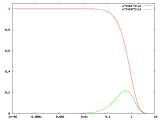
\includegraphics{bess.png}
      \end{center}
      \caption{\label{fig:bess} The zero and first order modified Bessel functions. }
    \end{wrapfigure}
    In Eq.~\ref{eq:fourier3tmp}, $E_{y}$ carries an additional factor of 
      $\gamma$ in the numerator relative to the $E_{x}$.
    $E_{y}$ is $\gamma$ times larger then $E_{x}$.

    In the ultra-relativistic limit, the electric and magnetic fields have the 
      same configuration as electromagnetic plane wave radiation. 
    The electric and magnetic fields are perpendicular and related by a factor
      of $c$ in the ultra relativistic limit.
    When $v$ approaches $c$, $\beta \approx 1$, the y-component of the 
      electric field and the z-component of the magnetic field are related by 
      a factor of $c$, $E_{y}/c=B_{z}$.
    Because $K_{0}(x)$ is smaller than $K_{1}(x)$ for all x, when $\gamma >> 1$, 
      $E_{y}$ is approximately equally to $\gamma$ $E_{x}$. 
    The conditions imposed by the ultra-relativistic limit result in the 
      relationship of Eq.~\ref{eq:ultraRelAprox}.
    \begin{equation} \label{eq:ultraRelAprox}
      \gamma >> 1 \rightarrow \gamma E_{x}>>E_{x} \rightarrow E_{y} >> E_{x}
    \end{equation}
    The x-component of the electric field can therefore be ignored and 
      the magnetic and electric fields are left perpendicular to each other.
    The six field components reduced to one electric component and one 
      perpendicular magnetic field component, which have a configuration 
      identical to a plane wave. 

    As with plane waves, the energy per area per time transfered by 
      the electromagnetic field is given by the Poynting vector.
    The Poynting vector takes the simple form of a plane pulse propagating in 
     the x direction.
    \begin{equation} \label{eq:poyntingVectortmp}
        \vec{\mathbf{S}}\equiv
	\vec{\mathbf{E}}\times\vec{\mathbf{B}}/\mu_{0}=
	\left(E_{y}^{2}/c\mu_{0}\right)\mathbf{\hat{x}}=
	c\epsilon_{0}E_{y}^{2}\mathbf{\hat{x}}
    \end{equation}
    The Poynting vector relates to the fluence (energy per unit area) 
      \cite{WWBrau},
    \begin{equation} \label{eq:fluencytmp}
        I(b)=\mathbf{\hat{x}}\cdot\int^{\infty}_{0}\vec{\mathbf{S}}d\omega=
	 \int^{\infty}_{0}\left(c\epsilon_{0}E_{y}^{2}\right)d\omega=
	 \int^{\infty}_{0}\left(\frac{dI}{d\omega}\right)d\omega
    \end{equation}
      and the spectral fluence (energy per area per frequency).
    \begin{equation} \label{eq:specturalFluencytmp}
	\frac{dI}{d\omega}=c\epsilon_{0}E_{y}^{2}=
	 \frac{e^{2}Z^{2}c}{4\pi^{3}b^{2}v^{2}\epsilon_{0}}
	 \left(\frac{\omega b}{\gamma v}\right)^{2}
	 K_{1}^{2}\left(\frac{\omega b}{\gamma v}\right)=
	\alpha\hbar\left(\frac{Z}{b\beta\pi}\right)^{2}
	 \left(\frac{\omega b}{\gamma v}\right)^{2}
	 K_{1}^{2}\left(\frac{\omega b}{\gamma v}\right)
    \end{equation}
    Substituting Eq.~\ref{eq:fourier3tmp} into Eq.~\ref{eq:fluencytmp} gives 
      the Poynting vector as a function of frequency.
    Eq.~\ref{eq:specturalFluencytmp} paves the way for Einstein's 
      equation. 
    The spectral fluence given by Eq.~\ref{eq:specturalFluencytmp} 
      relates the frequency to energy, which are the same quantities 
      present in Einstein's equation. 

    Einstein's equation, $E=\hbar\omega$, gives the energy of a photon, which
      is related to the spectral fluence. 
    If the fluence is due to a photon number density, $N$, Einstein's equation
      relates $N$ to the fluence. 
    The relationship between the number of photons per unit area in an 
      infinitesimal energy range and the spectral fluence in an infinitesimal 
      frequency range is given by Eq.~\ref{eq:photonFluxtmp} \cite{WWJackson}.
    \begin{equation}  \label{eq:photonFluxtmp}
        \frac{dI}{d\omega}d\omega=\hbar\omega N(\omega)d(\hbar\omega)
         \rightarrow \frac{1}{\hbar^{2}\omega}\frac{dI}{d\omega}=N(\omega)
    \end{equation}
    Plugging Eq.~\ref{eq:specturalFluencytmp} into 
      Eq.~\ref{eq:photonFluxtmp} yields the semiclassical photon flux of an 
      ultra-relativistic nucleus.
    \begin{equation} \label{eq:photonFluxFinaltmp}
	N(\omega,b)=\frac{\alpha}{\hbar\omega}
	 \left(\frac{Z}{b\beta\pi}\right)^{2}
	 \left(\frac{\omega b}{\gamma v}\right)^{2}
	 K_{1}^{2}\left(\frac{\omega b}{\gamma v}\right)
    \end{equation}
    Eq.~\ref{eq:photonFluxFinaltmp} replaces the classical electric field of a 
      point charge with a semiclassical field of photons. 
    Physicists can calculate the electromagnetic interactions between nuclei 
      with the final result of the Weizs\"{a}cker-Williams approximation, 
      Eq.~\ref{eq:photonFluxFinaltmp}.
    The photon flux in Eq.~\ref{eq:photonFluxFinaltmp} provides the 
      electromagnetic input to the $J/\psi$ photoproduction cross section 
      calculation. 


  \section{\label{sec:vdmTheory}Vector Meson Dominance}
    The Vector Messon Dominace method for calculating the $J/\psi$
      photoproduction cross section has three main components.
    VMD approach is constructed from the Weizsi\"{a}cker-Williams photon
      flux, the VMD fit to the proton-electron data, and the Glauber model for 
      calculating the nuclear cross sections from the proton-electron cross 
      sections.
    The Weizsi\"{a}cker-Williams photon flux provides the probe. 
    The proton-electron scattering data combine with the Glauber model  
      create a picture of the initial state of the nucleus. 
    Each of the different approaches to calculating the UPC $J/\psi$ 
      photoproduction cross section use these same elements.
    However, the different models each use the last two elements differently 
      to produce different pictures of the nucleus and different cross 
      sections values. 

    The photon flux in the photoproduction cross section calculation must be 
      finite in order for the cross section to be meaningful.
    The Weizsi\"{a}cker-Williams approximation, Eq.~\ref{eq:photonFluxFinaltmp}, 
      produces a divergence at $b=0$.
    The probability of the nuclei interacting would exceed one if the photon 
      flux were infinite. 
    The divergence that arises at $b=0$ from $K_{1}$ results in an 
      unphysically infinite photon flux.
    Removing the divergence is necessary.
    Special treatment of impact parameter, $b$, where the colliding nuclei 
      overlap eliminates the divergence. 
    
    A modulation of the photon flux can subdue the divergence at $b=0$.
    A convolution of the photon flux with the nucleon number density functions 
      of the colliding nuclei produces the necessary modulation. 
    Eq.~\ref{eq:woodsSaxon} gives the nucleon density of a single nucleus,
    \begin{equation} 
      \rho_{A}(s)=\frac{\rho_{0}}{1+exp[(s-R_{WS})/d)]}
      \label{eq:woodsSaxon}
    \end{equation}
    In Eq. ~\ref{eq:woodsSaxon}, $s$ is the distance from the center of the 
      nucleus, $R_{WS}$ is the radius of the nucleus, and $d$ is the skin depth, 
      which determines how quickly the nucleon density falls off beyond the 
      nuclear radius. 
    In Eq.~\ref{eq:TaNuc} the depth of the nucleus is integrated out leaving
      just the transverse dimension in $T_{A}$.
    The average number of nucleons in the overlap region is given by a 
      convolution of $T_A$ from each of the two nuclei to produce $T_{AA}$.
    \begin{eqnarray} \label{eq:TaNuc}
      T_{A}(\vec{r})=\int{dz\rho_{A}(\sqrt{|\vec{r}|^{2}+z^{2}})} \nonumber \\ 
      T_{AA}(|\vec{b}|)=\int{d^{2}\vec{r}T_{A}(\vec{r})T_{A}(\vec{r}-\vec{b})}
    \end{eqnarray}
    $T_{AA}$ is the function that modulates the photon flux. 
    As input to the Poisson distribution, $T_{AA}$ reduces 
      Eq.~\ref{eq:photonFluxFinaltmp} at values of $b$ where the nuclei overlap 
      significantly and eliminates the divergence in the photon flux. 
    
    Modulating the photon flux by the probability that no nucleon-nucleon 
      collisions occur limits the photon flux at low $b$ in Eq.~\ref{eq:photonFluxFinaltmp}.
    The convolution of the photon flux with the $b$ dependent probability that 
      no nucleon-nucleon collisions occur removes the divergence in 
      Eq.~\ref{eq:photonFluxFinaltmp}. 
    Using the mean number of nucleons in the overlap region given by $T_{AA}$, 
      the Poisson distribution gives the probability that no collisions 
      occur at a given $b$:
    \begin{equation} \label{eg:poisNoCol}
      P_{0}(b)=exp[-T_{AA}(b)\sigma_{NN}]
    \end{equation}
    In Eq.~\ref{eg:poisNoCol}, $\sigma_{NN}$ is the cross section for a 
      nucleon-nucleon interaction, which gives the probability that a collision
      will occur given the average number of nucleons in the overlap region.
    The average photon flux over impact parameter, $b$, can be calculated 
      from the integration of the $b$-dependent photon flux, Eq.~\ref{eq:photonFluxFinaltmp}, 
      with the $b$-dependent probability of having no nucleon-nucleon 
      interactions, Eq.~\ref{eg:poisNoCol}. 
    \begin{equation} \label{eq:fluxMod}
      \frac{dN_{\gamma}(k)}{dk}=\int_{0}^{\infty}{2\pi bdbP_{0}(b)
         \int_{0}^{R}{\frac{rdr}{\pi R^{2}_{A}}\int_{0}^{2\pi}d\phi
         \frac{d^{3}N_{\gamma}(k,b+r\cos(\phi))}{dkd^{2}r}}}
    \end{equation}
    Eq.~\ref{eq:fluxMod} goes down to $b=0$ where the photon flux is infinite, but 
      because the probability of having a nucleon-nucleon collisions is high, 
      the divergence is eliminated.
    The result of Eq.~\ref{eq:fluxMod} does not diverge.  

    A power-law fit to the proton photoproduction data gives an analytic 
      expression for the energy dependence of the proton photoproduction 
      cross section.
    The fitting function is simple and only depends on the photon-proton center
      of mass energy, $W$. 
    Eq.~\ref{eq:proElFit} gives the parameterization of the forward 
      proton photoproduction cross section fit. 
    \begin{equation} \label{eq:proElFit}
      \frac{d\sigma(\gamma p\rightarrow Vp)}{dt}\Big|_{t=0}
        =b_{v}(XW^{\epsilon}+YW^{-\eta})
    \end{equation}
    $W$ is the center of mass energy of the proton-photon system in 
      Eq.~\ref{eq:proElFit}.
    The remaining variables in Eq.~\ref{eq:proElFit} are simple power-law fit
      parameters.  
    The $XW^{\epsilon}$ term characterizes pomeron mediated interactions, and
      the $YW^{\eta}$ term characterizes meson mediated interactions\cite{vmd1999}. 
    $J/\psi$'s high mass relative to the $\pi$ and $\rho$ renders the second 
      term in Eq. ~\ref{eq:proElFit} negligible as the term falls rapidly with
      increasing $W$. 
    Eq.~\ref{eq:proElFit} allows for extrapolation and interpolation of the 
      measured forward proton photoproduction cross section. 
    The fit to the data provides estimates for energies that have not yet been 
      probed experimentally.

    The proton-electron scattering data is used differently in the VMD method 
      than in the other major methods.  
    The VMD method for calculating UPC photoproduction cross sections 
      relies more on electron-proton scattering data.
    The proton photoproduction cross sections from the electron-proton 
      scattering data is a direct input to the VMD model. 
    A power-law fit to the proton photoproduction data, as opposed to model 
      dependent gluon densities of other approaches, combines with the Glauber
      model to provide the nuclear model in the VMD method. 
    Because of the simplicity of the method, the VMD approach incorporates less
      modifications of the nuclear initial state relative to the proton initial
      state. 
    As a result, the VMD method produces a higher UPC J/$\psi$ photoproduction 
      cross section relative to the other methods. 

    Vector meson dominance and the optical theorem allow for the calculation of 
      the total proton-meson scattering cross section from the fit given by 
      Eq.~\ref{eq:proElFit}. 
    The optical theorem relates a total cross section, $\sigma$, 
      to a corresponding forward scattering cross section, $d\sigma/dt|_{t=0}$.
    Vector meson dominance asserts that the colored part of the photon wave 
      function is dominated by vector mesons; therefore, the photon is 
      represented as a quark-antiquark pair in photoproduction calculations. 
    These two components combine to produce Eq.~\ref{eq:VMDforwardScat}.
    \begin{eqnarray} \label{eq:VMDforwardScat}
      \frac{d\sigma(\gamma p\rightarrow Vp)}{dt}\Big|_{t=0}=
        \frac{4\pi \alpha}{f^{2}_{v}(M_{V},\Gamma_{l^{+}l^{-}})}\frac{d\sigma(Vp\rightarrow Vp)}{dt}
        \Big|_{t=0} \nonumber \\
       \sigma(Vp)_{tot}^{2}=16\pi\frac{d\sigma(Vp\rightarrow Vp)}{dt}\Big|_{t=0}
    \end{eqnarray}
    In Eq.~\ref{eq:VMDforwardScat}, the photon-proton scattering is related to
      meson-proton scattering through the photon-meson coupling, which 
      depends on the vector meson's mass, $M_{V}$, and leptonic decay width, 
      $\Gamma_{l^{+}l^{-}}$. 
    The result of combining vector meson dominance and the optical theorem 
      in Eq.\ref{eq:VMDforwardScat} provides the cross section for a meson to 
      scatter off a proton.
    The total proton-meson scattering cross section, provides 
      the input to the Glauber model calculation of the nuclear photoproduction 
      cross section. 

    The nucleus-meson scattering cross section relates to 
      Eq.~\ref{eq:VMDforwardScat} through the Glauber model. 
    The Glauber model allows for Eq.~\ref{eq:VMDforwardScat}, the proton-meson
      scattering cross section, to be used to calculate a nucleus-meson 
      scattering cross section. 
    The Glauber model produces nuclear cross section calculations from 
      nucleon (proton or neutron) interaction cross sections by use of $T_{AA}$. 
    The combination of the mean number of nucleons in the overlapping region
      of a nucleus-nucleus collision, $T_{AA}$, the nucleon cross section, 
      $\sigma$, and the Poisson distribution make-up the core of the Glauber 
      model. 
    For the total nucleus-meson scattering cross section, the equation has the 
      following form:
    \begin{equation} \label{eq:glauber}
      \sigma_{tot}(VA)=\int d^{2}\vec{r}(1-e^{-\sigma_{tot}(Vp)T_{AA}(\vec{r})})
    \end{equation}
    In Eq.~\ref{eq:glauber}, the term $e^{\sigma_{tot}(Vp)T_{AA}}$ gives the
      probability of having no meson-nucleon scatterings from the Poisson 
      distribution. 
    The probability of having at least one scattering is given by subtracting 
      one from the term  $e^{\sigma_{tot}(Vp)T_{AA}}$ in Eq.~\ref{eq:glauber}.
    As seen in Eq.~\ref{eq:glauber}, the Glabuer model leverages scientific 
      knowledge of the proton to understand of the nucleus. 
    The Glauber model is the tool that combines the proton photoproduction data 
      with nucleon distributions in the nucleus to produce a nuclear vector 
      meson photoproduction cross section in the VMD approach. 

    Reversing the process used for the proton, Eq.~\ref{eq:glauber}, the meson 
      nucleus scattering cross section, relates to forward nuclear 
      photoproduction cross section through the optical theorem. 
    The nuclear photoproduction cross section is the input to the calculation 
      of the final result, the nuclear vector meson photoproduction cross 
      section in UPC events.  
    Eq.~\ref{eq:optTheA} uses the optical theorem to produce the nuclear 
      photoproduction cross section from the nucleus-meson scattering cross 
      section:
    \begin{eqnarray} \label{eq:optTheA}
      \frac{d\sigma(\gamma A\rightarrow VA)}{dt}\Big|_{t=0}=
      \frac{\alpha\sigma_{tot}^{2}(VA)}{4\pi f_{v}^{2}}\nonumber \\
      \sigma(\gamma A\rightarrow VA)=\frac{d\sigma(\gamma A\rightarrow VA)}{dt}
        \Big|_{t=0}\int_{t_{min}}^{\infty}dt|F(t)|^{2}
    \end{eqnarray}
    $F$ in equation Eq.~\ref{eq:optTheA} is the Fourier transform of the 
      nuclear density function, $\rho_{A}$.
    To produce the formula for calculating the UPC vector meson 
      photoproduction cross section, Eq.~\ref{eq:optTheA} is combined with the 
      photon flux incident on the nucleus, Eq.~\ref{eq:fluxMod}. 
    \begin{equation} \label{eq:finalVMDResult}
      \sigma(AA\rightarrow AAV)=2\int{dk\frac{dN_{\gamma}}{dk}
                    \sigma(\gamma A\rightarrow VA)}
    \end{equation}
    The factor of 2 in Eq.~\ref{eq:finalVMDResult} comes from the fact that both 
      of the two colliding nuclei contribute. 
    Combining the three elements of VMD, Eq.~\ref{eq:finalVMDResult} is the 
      final result of the VMD UPC photoproduction cross section calculation. 
    Vector meson production rates in UPC collisions are predicted 
      by Eq.~\ref{eq:finalVMDResult}, which can be confirmed or denied by 
      experiment. 


      \section{\label{sec:ltaTheory}Leading Twist Approach Derivation}
    The LTA method for calculating UPC photoproduction cross sections
      combines elements of the Glauber model with direct use of gluon 
      densities. 
    The proton gluon density is modified by a nuclear modification 
      function in the LTA method to produce the nuclear gluon density. 
    The nuclear modification function converts the proton photoproduction
      cross section to a nuclear photoproduction cross section in the LTA 
      method.
    The LTA method is different from the other methods in its direct use of the
       nuclear modification factor and how the nuclear modification factor
       calculation incorporates multiple scattering.
    The direct use of the nuclear modification factor produces the most gluon 
      shadowing out of the three major methods, and results in the lowest
      cross sections.
    The LTA method is the easiest to constrain experimentally for this reason. 

    The LTA method uses the Weizsi\"{a}cker-Williams approximation to calculate 
      the photon flux created by the colliding nuclei. 
    As in the VMD method, the probability of having no hadronic collisions 
      modulates the flux.
    The photon flux for the LTA method has the following form \cite{lta2011.09}:
    \begin{eqnarray} \label{eq:ltaPhotonFlux}
      n_{\gamma/A}^{i}(\omega_{\gamma})=\frac{2\alpha Z^{2}}{\pi}\int_{b_{min}}^{\infty}
        db\frac{x^{2}}{b}\Big[K_{1}^{2}(x)+\frac{K_{0}^{2}(x)}{\gamma_{L}^{2}}\Big]
        P_{0}(b)P_{C}^{i}(b) \\
      x=\frac{\omega b}{\gamma_{L} v} \nonumber 
    \end{eqnarray}
    The $K_{0}^{2}(x)$ term contributes a photon flux in the 
      transverse direction.
    $P_{C}^{i}(b)$ is an additional modulation factor that requires various 
      additional interactions. 
    These interactions result in additional emissions of neutrons from the 
      receding nuclei as the nuclei relax from excited states. 
    The LTA flux reproduces the VMD result when the $K_{0}$ term becomes 
      negligible as $\gamma_{L}$ approaches $\infty$ and $P_{C}^{i}=1$ when all
      emissions are allowed.
    The terms $P_{C}^{i}$ and $K_{0}$ create additional ways to distinguish UPC
      events from nuclear collisions experimentally but leave the underlying 
      interaction mechanism the same. 
    For example, the additional terms in the LTA formulation of the photon flux
      produce calculations of asymmetric neutron emission, which separate UPC 
      events from nuclear collisions.  

    The LTA method calculates the nucleon photoproduction cross section 
      from the nucleon gluon density. 
    Ref. \cite{lta2011.09} derives the nucleon cross section from derivations
     of the nucleon gluon densities from electron-proton scattering data and
     leading order perturbative quantum field theory calculations.
    The forward photoproduction cross section of the nucleon has the following
     form \cite{lta2011.09}:
   \begin{equation} \label{eq:ltaFowardPhotoXSec}
     \frac{d\sigma_{\gamma N\rightarrow J/\psi N}(t=0)}{dt}=\frac{16\Gamma_{l^{+}l^{-}}\pi^{3}}
     {3\alpha M_{J/\psi}^{5}}[\alpha_{s}\mu^{2}xG_{N}(x,\mu^{2})]^{2}
   \end{equation}
   Here $G_{N}$ is the gluon density of the nucleon, $x$ is the fraction of
     the nucleon's momentum the gluon carries, and $\mu$ is related
     to momentum at which the nucleon is being probed, which is equal to 
     $M_{J/\psi}/2$ for $J/\psi$ photoproduction.
   In Eq.~\ref{eq:ltaFowardPhotoXSec} the nucleon cross section is explicitly 
     connected to the gluon density.
   By connecting the gluon density to the cross section, Eq.~\ref{eq:ltaFowardPhotoXSec}
     allows for the gluon density to be experimentally probed. 

   Ref. \cite{lta2011.09} exploits the optical theorem to relate the forward 
     photoproduction cross section of the nucleon to the nuclear cross section. 
   Eq.~\ref{eq:ltaOptTheWNucMo} gives the relation:
   \begin{eqnarray} \label{eq:ltaOptTheWNucMo}
     \sigma_{\gamma A\rightarrow J/\psi A}(\omega)=
     \frac{d\sigma_{\gamma N\rightarrow J/\psi N}}{dt}(\omega,t_{min})
     R_{g}^{2}\int_{t_{min}}^{\infty}dt|F(t)|^{2} \\
     R_{g}=\frac{G_{A}(x,\mu^{2})}{AG_{N}(x,\mu^{2})} \nonumber 
   \end{eqnarray} 
   $R_{g}$, the nuclear modification function, is the ratio between the gluon 
     density of the nucleon, $G_{N}$, to the gluon density of the nucleus, 
     $G_{A}$.
   As with the VMD method, the optical theorem relates the forward cross 
     section, $\frac{d\sigma_{\gamma N\rightarrow J/\psi N}}{dt}(\omega,t_{min})$,
     to the total cross section, $\sigma_{\gamma A\rightarrow J/\psi A}$. 
   The LTA method relates the measurable UPC photoproduction cross section 
     to the gluon density of the nucleus.  
   Eq.~\ref{eq:ltaOptTheWNucMo} further connects the gluon density of the 
     nucleon to the relative reduction of the gluon density in the nucleus 
     through $R_{g}$.

   From Eq.~\ref{eq:ltaOptTheWNucMo}, the LTA method can predict the angular 
     distribution of photoproduced $J/\psi$ with respect to the beam axis. 
   In Ref. \cite{lta2012.03} the angular distribution is expressed in the form 
     of the rapidity dependency of the UPC photoproduction cross section. 
   \begin{eqnarray} \label{eq:ltaRapDist}
     \frac{d\sigma_{A_{1}A_{2}\rightarrow A_{1}A_{2}J/\psi}}{dy}=
       n_{\gamma/A_{1}}(y)\sigma_{\gamma A_{2}\rightarrow J/\psi A_{2}}(y)
       +n_{\gamma/A_{2}}(-y)\sigma_{\gamma A_{1}\rightarrow J/\psi A_{1}}(-y) \\
       y=ln\Big(\frac{2\omega}{M_{J/\psi}}\Big) \nonumber
   \end{eqnarray}
   Eq.~\ref{eq:ltaRapDist} is comprised of two terms, one for photons from the
     forward going nucleus interacting with the backward going nucleus, and 
     a second for the reverse situation. 
   The integration of Eq.~\ref{eq:ltaRapDist} over $y$ produces the factor of 2 
     that is present in Eq.~\ref{eq:finalVMDResult}.
   The rapidity distribution of the photoproduction cross section given in 
     Eq.~\ref{eq:ltaRapDist} provides a more detailed prediction and allows for
     more direct experimental comparison.
   Eq.~\ref{eq:ltaRapDist} allows for comparison to rapidity regions that are 
     covered by experiments.
  
   The LTA method is distinct from the pQCD method and VMD method through the 
     use $R_{g}$, the nuclear gluon modification factor. 
   As opposed to using $R_{g}$, the pQCD method uses the nuclear gluon 
     density, and VMD model uses proton photoproduction cross sections 
     directly. 
   In the LTA method, $R_{g}$ is calculated through a combination of $J/\psi$ 
     photoproduction data from proton-electron scattering and DGLAP evolution 
     equations, which incorporates nuclear multiple scattering effects 
     \cite{lta2011.09}. 
   The DGLAP evolution equations give the depends of nuclear gluon densities on
     the momentum scale at which the nucleus is probed, $\mu$ in 
     Eq.~\ref{eq:ltaFowardPhotoXSec}. 
   The unique way the LTA method calculates $R_{g}$ results in lower cross 
     sections than the other major methods and allows for experimental
     sensitivity. 
   Experimental measurements of the UPC $J/\psi$ photoprodcution cross section 
     with CMS have the opportunity to distinguish whether $R_{g}$ as calculated 
     in the LTA method accurately predicts the gluon density of the nucleus. 
  
 
  \section{Perturbative Quantum Chromo-dynamics}
    To calculate the UPC $J/\psi$ photoproduction cross section, the pQCD 
      method uses the nuclear gluon density to characterize the nucleus and 
      the Weizs\"{a}cker-Williams approximation for the probing photon flux. 
    The pQCD method combines these components such that the nuclear gluon 
      density is a direct variable.
    The nuclear gluon density term in the pQCD formulation allows for 
      the use of a variety of nuclear gluon density models.
    A range of nuclear gluon densities are present in the available models
      resulting in a wide range of cross section values. 
    The UPC $J/\psi$ photoproduction cross section is correlated with the gluon
      density of the nucleus rising with higher densities and shrinking with 
      lower densities. 
    In the pQCD approach, the calculation of the UPC $J/\psi$ photoproduction 
      cross section allows experiments to constrain many different nuclear 
      gluon density models. 
    
    In the pQCD method, the photon interacts with the nucleus by fluctuating to 
      a quark-anitquark pair.
    For $J/\psi$, the photon fluctuates to a $c\bar{c}$ pair. 
    The probability for the photon to fluctuate to a $c\bar{c}$ pair
      depends on the $M_{J/\psi}$, the mass of $J/\psi$, $\Gamma_{l^{+}l^{-}}$, 
      the $J/\psi$ leptonic decay width, and $\alpha$, the electromagnetic 
      coupling constant.
    These three variables connect the c quark to the electromagnetic force 
      mediator, the photon. 
    Recast as a $c\bar{c}$ pair, the photon couples to the nuclear gluon 
      density.
    Ref. \cite{pQCD2011.08} uses the fluctuation of the photon to a $c\bar{c}$ 
      pair as the foundation for calculating the forward $J/\psi$ 
      photoproduction cross section. 

    The $c\bar{c}$ pair arising from the photon fluctuation scatters off the 
      gluons of the nucleus. 
    The density of gluons in the nucleus determines how likely and therefore 
      how large the cross section is for the quarks to scatter and form a 
      $J/\psi$.
    The forward scattering cross section is the portion of those scattering 
      events which transfer the minimum amount of momentum between the 
      photon and the nucleus. 
    The forward cross section for $J/\psi$ photoproduction in the nucleus has 
      the following form \cite{pQCD2011.08}:
    \begin{equation} \label{eq:pQCDfowardScat}
      \frac{d\sigma_{\gamma A\rightarrow J/\psi A}}{dt}\Big|_{t=0}=\xi_{J/\psi}
        \Big(\frac{16\pi^{3}\alpha_{s}^{2}\Gamma_{l^{+}l^{-}}}{3\alpha 
        M_{J/\psi}^{5}}\Big)[xG_{A}(x,\mu^{2})]^{2}
    \end{equation}
    In Eq.~\ref{eq:pQCDfowardScat}, $\xi_{J/\psi}$ is an experimentally derived 
      correction factor, $\alpha_{s}$ is the strong coupling constant, $x$ is 
      the momentum faction of the nucleus the scattering gluons carry, and 
      $G_{A}$ is the gluon density of the nucleus. 
    Both the $c$ and $\bar{c}$ couple to the gluon density, and the double 
      coupling results in the squared dependence of the cross section on the 
      gluon density in Eq.~\ref{eq:pQCDfowardScat}. 
    Fitting Eq.~\ref{eq:pQCDfowardScat} to proton-electron scattering data 
      sets $\xi_{J/\psi}$ \cite{pQCD2011.08}.
    The forward scattering cross section given by Eq.~\ref{eq:pQCDfowardScat} 
      connects the photon flux to the gluon density and provides the input to 
      calculate the total cross section by the optical theorem. 
    Eq.~\ref{eq:pQCDfowardScat} is the crux of how UPC measurements provide
      insight into the gluon content of the nucleus.
    
    The optical theorem relates the forward cross section in 
      Eq.~\ref{eq:pQCDfowardScat} to the total photoproduction cross section. 
    The total cross section calculated by use of the optical theorem gives 
      the probability that a photon incident on the nucleus will produce a 
      $J/\psi$ regardless of the momentum transfered in the interaction. 
    Ref. \cite{pQCD2011.08} gives the form of the total cross section equation:
    \begin{equation} \label{eq:pQCDtotXSec}
      \sigma_{\gamma A\rightarrow J/\psi A}(k)=
      \frac{d\sigma_{\gamma A\rightarrow J/\psi A}}{dt}\Big|_{t=0}
      \int_{t_{min}(k)}^{\infty}dt|F(t)|^{2}
    \end{equation} 
    Here $t_{min}=(M_{J/\psi}^{2}/4k\gamma_{L})^2$, which is the minimum amount
      of momentum transfer required to produce a $J/\psi$ given the photon wave
      number $k$.
    The $k$ dependence of $t_{min}$ produces the rapidity, $y$, dependence of
      the total cross section.
    The total cross section for photoproduction, Eq.~\ref{eq:pQCDtotXSec}, 
      provides the input to Eq.~\ref{eq:ltaRapDist}, 
      which gives the rapidity dependence of the UPC photoproduction cross 
      section. 
    Eq.~\ref{eq:pQCDtotXSec} as input to Eq.~\ref{eq:ltaRapDist} allows for 
      experimental comparison of the pQCD method to measurements of UPC 
      photoproduction cross sections. 
    With the pQCD method's direct use of the nuclear gluon density in 
      Eq.~\ref{eq:pQCDfowardScat}, the pQCD method allows for experimental 
      exploration of any gluon density model. 


  \section{Incoherent Photoproduction}


  \section{Photon Induced Nuclear Break-up}


  \section{Theoretical Results}
  The UPC photoproduction cross section calculations depend significantly on 
    how the nucleus is represented in the calculation. 
  The results from the VMD, LTA, and pQCD methods vary from a relatively 
    large cross section in the VMD model, ranging through a variety of values
    in the pQCD method, to a relatively small cross section in the LTA method. 
  Each of these methods utilizes the same probe of the nucleus, the equivalent 
    photon flux that is calculated using the Weizsi\"{a}cker-Williams approximation. 
  The three methods deviate in how they calculate the forward photoproduction
    scattering cross section.
  The differences in the UPC photoproduction cross sections predicted by the 
    different models demonstrates the amount of experimental sensitivity there 
    is to distinguishing between the models. 
  The dependence of the cross section on rapidity shows where in phase space 
    a measurement of the cross section is most sensitive.
   
  The predicted value for the UPC $J/\psi$ photoproduction cross section in 
    PbPb collisions at the LHC differ widely depending on which of the three 
    main methods is used. 
  The cross section value calculated by Eq.~\ref{eq:finalVMDResult} in the 
    VMD, LTA, and the various gluon density models in pQCD method vary 
    significantly.
  Table~\ref{tab:allXsec} gives the predicted values for the three main methods
    taken from Ref~\cite{pQCD2013.02}, Ref~\cite{lta2011.09}, and Ref~\cite{vmd1999}.
  \begin{table} 
   \centering
   \begin{tabular}{|l|l|} 
     \hline
     Model & $\sigma_{AA\rightarrow AAJ/\psi} (mb)$ \\ \hline \hline
     VMD/STARlight MC & 23 \\ \hline
     LTA & 9 \\ \hline
     pQCD-MSTW08 & 34 \\ \hline
     pQCD-EPS08 & 7  \\ \hline
     pQCD-EPS09 & 14 \\ \hline
     pQCD-HKN07 & 23 \\ \hline
     \hline
   \end{tabular}
   \caption{$\sigma_{AA\rightarrow AAJ/\psi} (mb)$
    the LTA, VMD, pQCD methods. Four different gluon density models are used 
    in the pQCD method. STARlight is a simulation software package that utilizes 
    the VMD model.}
   \label{tab:allXsec}
  \end{table}
  The cross sections in Table~\ref{tab:allXsec} differ by a factor of $\approx4$ 
    from the smallest to largest and create an experimental opportunity. 
  The clear discrepancy between the models in Table~\ref{tab:allXsec} 
    demonstrates the high amount of experimental sensitivity there is for 
    distinguishing between the models. 

  The rapidity dependence of the cross sections determine which values of 
    rapidity will be most sensitive to differences in the models. 
  The rapidity dependence calculated by Eq.~\ref{eq:ltaRapDist} overlap between 
    the models at certain values of $y$ leaving the models indistinguishable at
    that rapidity.
  Fig.~\ref{fig:rapDepAll} \cite{alice2012.09} shows the rapidity dependency of 
    the UPC $J/\psi$ photoproduction cross section for the three main models 
    including several different gluon density models using the pQCD method.
  \begin{figure}[h] 
    \begin{center}
      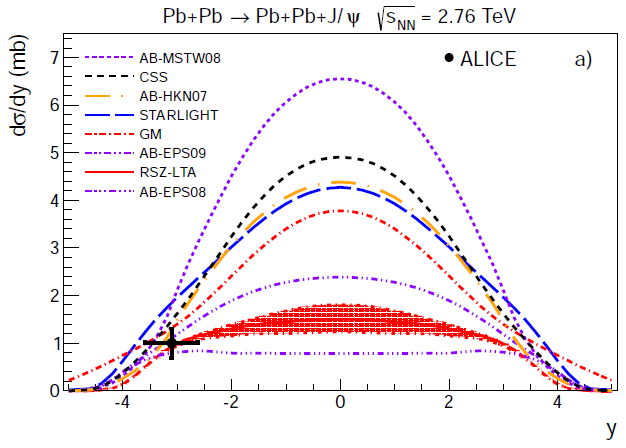
\includegraphics[width=0.5\textwidth,keepaspectratio]{aliceDsigDy.png}
    \end{center}
    \caption{ \label{fig:rapDepAll} AB is the pQCD method, RSZ-LTA is the LTA method, and STARlight
      is the VMD model.}
  \end{figure}
  In Fig.~\ref{fig:rapDepAll} at higher rapidities, in particular $|y|>3$, the 
    various models give similar values for $d\sigma/dy$. 
  At $y=0$ the models vary the most. 
  Fig.~\ref{fig:rapDepAll} shows that experiments that can measure $J/\psi$
    at $y=0$ have the best opportunity to distinguish between the models.
  The high sensitivity at $y=0$ creates an advantage for experiments that can 
    measure particles with small rapidity and low momentum.  
 
  The UPC photoproduction models each have different shapes to their rapidity 
    dependence. 
  The slope of $d\sigma/dy$ in Fig.~\ref{fig:rapDepAll} depends on the model. 
  Through the rapidity region $1<|y|<3$, each of the models has a progressively
    steeper slope. 
  The LTA method and the pQCD method utilizing the EPS08 gluon density model 
    are relatively flat where as the VMD and other gluon density models using
    the pQCD method have a noticeable slope.
  The differing slopes provide an additional experimental observable. 
  The shape of the rapidity distributions provide experimental sensitivity at 
    rapidities away from $y=0$ and creates an opportunity for experiments that 
    can not measure $J/\psi$ at $y=0$.

  The nuclear suppression factor, S, demonstrates the difference between how 
    the models represent the nucleus. 
  S, which is a ratio between the nuclear photoproduction cross section and the     
    free nucleon photoproduction cross seciton, is a measure of how the nuclear 
    gluon densities evolve in each of the models. 
  Fig.~\ref{fig:ltaAndPqcdNucSub} from Ref.\cite{lta2013.05} shows the nuclear 
    suppression, which is equivalent to $R_g$ in Eq.~\ref{eq:ltaOptTheWNucMo}, 
    for the LTA and pQCD method.
  \begin{figure}[h] 
    \begin{center}
      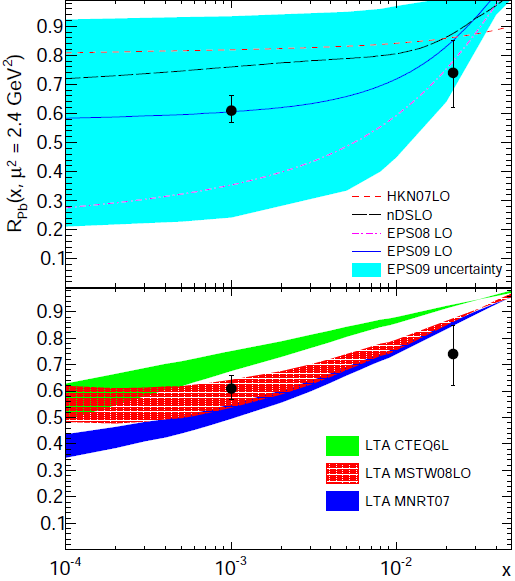
\includegraphics[width=0.5\textwidth,keepaspectratio]{ltaAndPqcdNucSub.png}
    \end{center}
    \caption{ \label{fig:ltaAndPqcdNucSub} Nuclear supression factor, $S$, in the pQCD and LTA methods.}
  \end{figure}
  \begin{figure}
    \begin{center}
      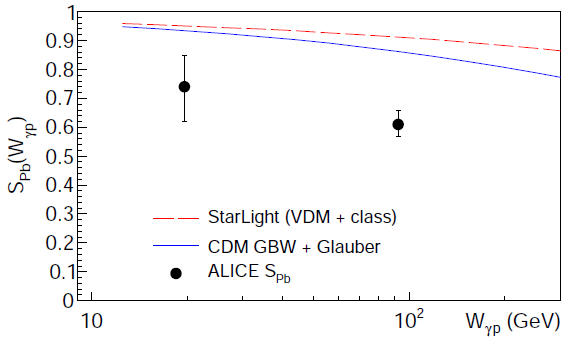
\includegraphics[width=0.5\textwidth,keepaspectratio]{ltaAndPqcdNucSubVMD.png}
    \end{center}
    \caption{ \label{fig:ltaAndPqcdNucSubVMD} Nuclear supression factor, $S$, in VMD method.}
  \end{figure}
  Fig.~\ref{fig:ltaAndPqcdNucSubVMD} shows the nuclear suppression for the VMD 
    method \cite{lta2013.05}. 
  Fig.~\ref{fig:ltaAndPqcdNucSubVMD} and Fig.~\ref{fig:ltaAndPqcdNucSub} show that 
    as the momentum of the probing photon goes up, increasing $W_{\gamma p}$, 
    and momentum of the probed gluon goes down, decreasing $x$, 
    the nuclear gluon density decreases relative to the free nucleon. 
  The nuclear suppression factor, S, allows for the different models' 
    representations of the gluon content of the nucleus to be directly compared
    to each other and to data. 
  S can be measured from data by assuming a Weizsi\"{a}cker-Williams photon flux and 
    provides insight into nuclear gluon densities. 
